\chapter{Materiais e Métodos} \label{cap:metod}

Nesse capítulo são descritos os métodos, assim como os materiais utilizados para o desenvolvimento deste trabalho. São descritas as etapas do projeto e os principais fundamentos e tecnologias a serem empregados.


\section{Materiais}
% arnaldo: 3.1 materiais: flutter, dart, python, mlkit, firebase, macbook para codificar (processador, memória, ...), software de emulação, iphone (geração, câmera, ...)
O ambiente de desenvolvimento da metodologia proposta se faz o uso de um Macbook Pro de 13 polegadas com processador Intel Core i5 de dois núcleos 2,3 GHz e memória integrada LPDDR3 de 8 GB com 2133 MHz e embarcado com o sistema operacional macOS Mojave versão 10.14.4.  

Para o desenvolvimento da metodologia, foi optado por utilizar as tecnologias de aplicativos móveis como Flutter, Dart, Python, OpenCV e Firebase MLKit devido às suas altas taxas de aprendizado e desempenho no desenvolvimento de aplicativos móveis.

O Flutter\footnote{https://flutter.dev/} foi construído pela Google com a finalidade de melhorar a qualidade dos aplicativos, a velocidade do desenvolvimento, e para alcançar mais usuários. Ele é um SDK  de código aberto para o desenvolvimento de aplicativos para Desktop, Web e dispositivos móveis como iOS e Android \cite{ARSTECHNICA2017}.


O Flutter é um poderoso \texttit{framework} porque o código é compilado em ARM, ou seja, compila o código para cada plataforma. Isso agiliza a abertura e o desempenho do aplicativo. Além disso, utiliza um renderizador Mobile First acelerado por GPU para que haja consistência da \texttit{UI} entre as plataformas e o dispositivo. Então o Flutter projeta os \texttit{widgets} com um \texttit{framework} personalizável e extensível em camadas \cite{IMASTERS}. Não há pontes entre o \texttit{framerwork} e os \texttit{widgets}, tornando a renderização eficiente. 

Flutter é escrito em Dart, uma linguagem concisa, fortemente tipificada e orientada a objetos. O Dart é bem semelhante à linguagens como Swift, C#, Java e JavaScript.

Python\footnote{https://www.python.org/} é uma linguagem de programação de alto nível, interpretada, de \texttit{script}, imperativa, orientada a objetos, funcional, de tipagem dinâmica e forte. Possui um modelo de desenvolvimento comunitário, aberto e gerenciado pela organização sem fins lucrativos Python Software Foundation \cite{PYTHON}.

Python será utilizado como ponte para o uso da biblioteca OpenCV (\texttit{Open Source Computer Vision Library}). O OpenCV é uma biblioteca multiplataforma, totalmente livre ao uso acadêmico e comercial, para o desenvolvimento de   aplicativos na área de Visão computacional. O OpenCV\footnote{https://opencv.org/}
possui módulos de Processamento de Imagens e Video I/O, Estrutura de dados, Álgebra Linear, GUI (Interface Gráfica do Usuário) básica com sistema de janelas independentes, controle de mouse e teclado, além de mais de 350 algoritmos de visão computacional como: filtros de imagem, calibração de câmera, reconhecimento de objetos, análise estrutural e outros \cite{RVOPENCV}. 

Para a extração dos caracteres da imagem será utilizado o SDK Firebase ML Kit\footnote{https://firebase.google.com/}, após a etapa de pré-processamento será testado a eficácia tanto da sua versão \texttit{online} quanto \texttit{offline}, para uma taxa maior de acertos nas palavras, diminuindo a complexidade da busca pelos registros na base de dados da ANVISA, disponibilizada em seu \texttit{site} oficial.

Os testes serão realizados pode meio do Android Device Manager, um simulador de iPhone X e um iPhone 7 físico. 

O Android Device Manager\footnote{https://developer.android.com/studio/run/managing-avds.html?hl=pt-br} é usado para criar e configurar AVDs (Dispositivos Virtuais Android) que são executados no Android Emulator. Cada AVD é uma configuração de emulador que simula um dispositivo Android físico. Assim, é possível executar e testar aplicativos em uma variedade de configurações que simulam diferentes dispositivos Android físicos  \cite{ADVDUNN}.

O simulador de iPhone está disponível na IDE de desenvolvimento da Apple, o Xcode\footnote{https://developer.apple.com/xcode/}, que funciona como um aplicativo separado por si só. É possível replicar de forma muito precisa a tela de um iPhone, iPad, Apple Watch ou Apple TV como uma janela na área de trabalho do Mac e é possivel manipular a tela e o aplicativo em execução com uma configuração de mouse e teclado \cite{IPHONESIMULATOR}.

Um iPhone 7 será utilizado como dispositivo físico  para testes, equipado com uma câmera de 12 MP com resolução de 1334x750 pixeis e abertura de abertura de ƒ/1.8, processador Quad-Core 2 GHZ, armazenamento de 128 GB e com sistema operacional iOS na versão 12.2.


\section{Métodos}
% arnaldo: 3.2 método: criar base (capturar imagens, dizer quantas imagens,  resolução, colorido, iluminação);  pré-processar para tirar as bordas e corrigir a perspectiva; ocr; buscar na base; vai ter algum pos-processamento (ex. corretor ortográfico para contorar falhas do ocr)
A base de imagens necessária para a realização deste trabalho será coletada por meio de capturas fotográficas com o auxílio de um iPhone 7 que dispõe de uma câmera de 12 MP e resolução de 1334x750 pixeis em uma farmácia da cidade Medianeira com uma boa iluminação ambiente. As imagens serão capturadas de 5 medicamentos aleatórios, e para que haja uma quantidade considerável de imagens, as imagens serão coletadas em diferentes perspectivas, distâncias entre câmera e área de interesse e tipos de fundo, totalizando então mais de 135 imagens coloridas padrão RGB.

A imagem em questão passará por seis etapas de pré-processamento com a utilização do OpenCV, conforme demonstrado na Figura~\ref{fig:diagrama}.

\begin{figure}[h!]
	\centering
	
	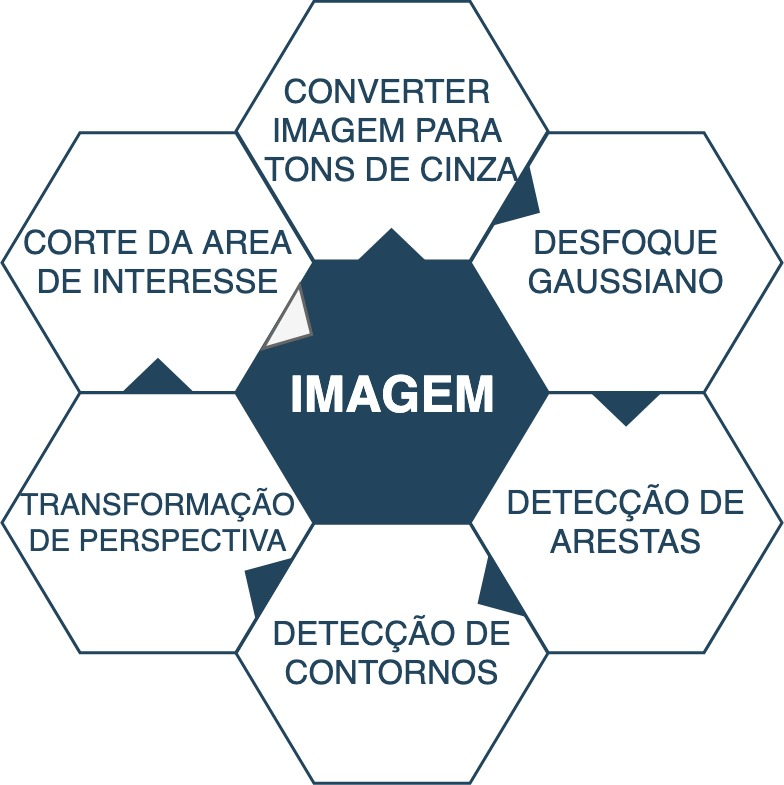
\includegraphics[width=0.5\textwidth]{Imagens/diagrama} 
	\caption[Etapas de pré-processamento da imagem.]{Etapas de pré-processamento da imagem.}
\fonte{Autoria própria.}	
	\label{fig:diagrama}
\end{figure}

Na primeira etapa, para que seja possível a detecção de arestas será necessário converter a imagem de RGB para escala de cinza, posteriormente é necessário aplicar um desfoque Gaussiano para remover ruído de alta frequência, para auxiliar na detecção de contorno na etapa seguinte e também na detecção de bordas Canny ou transformada de Hough. Aplicadas essas técnicas, é possível se obter um esboço em tons claros de cinza das arestas.

Como a região de interesse proposta pelo trabalho é uma caixa de remédio ou uma bula, é possível afirmar que a região de interesse é um retângulo e esse retângulo possui quatro arestas. Portanto, é possível criar uma heurística para a extração do contorno da área de interesse. A heurística supõe que o maior contorno da imagem com exatamente quatro pontos é a área de interesse a ser extraída. Esta suposição é razoavelmente segura, o problema assume que a região de interesse é o foco principal da imagem em análise e também deveria ser seguro afirmar que a área de interesse possui quatro contornos maiores, ignorando os contornos menores.

A próxima etapa é a aplicação da transformada de perspectiva, onde o objetivo é pegar os quatro pontos que representam o contorno do documento e aplicar uma transformação de perspectiva para obter uma ``vista aérea`` de cima para baixo da imagem.

Com a imagem já tratada, a última etapa do pré-processamento é o recorte da área de interesse já corrigida, substituindo a imagem original, para a extração de texto no OCR.

Após o reconhecimento dos caracteres, é possível que necessite a utilização de um corretor ortográfico para contornar falhas de reconhecimento do OCR. Será testado a eficácia do corretor ortográfico do Firebase ML Kit, que é um dicionário latino brasileiro. Caso o mesmo não venha atender as expectativas de contorno de falhas do OCR, será estudado outra opção de corretor ortográfico.

Para finalizar, as palavras encontradas estarão prontas para serem pesquisadas em uma base de dados extraída da ANVISA, para a projeção das informações do medicamento em interesse no aplicativo. 

A avaliação da eficácia da arquitetura em base do problema será feita em relação ao poder de acerto das palavras capturadas pelo OCR, comparando os resultados ao fazer testes unitários de cada método proposto no pré-processamento em ambos ambientes tanto offline quanto online.



% arnaldo: 3.3 avaliação: reconhecimento das palavras; conseguiu achar na base com as palavras detectadas na base da anvisa possível observar cada etapa em que a imagem percorre na metodologia desenvolvida.

